\documentclass[12pt]{article}
\usepackage{csquotes}
\usepackage{amsmath,amsfonts,amssymb}
\usepackage{geometry}
\usepackage{pifont}
\usepackage[utf8]{inputenc}
\usepackage[english]{babel}
\usepackage{ragged2e}
\usepackage{blindtext}
\usepackage[backend=biber, style=numeric]{biblatex}
\usepackage[hyperindex,breaklinks,colorlinks=true,linkcolor=blue,citecolor=blue,urlcolor=blue]{hyperref}
\usepackage{tikz}

\addbibresource{references.bib}
\addbibresource{references/DolevReference.bib}
\addbibresource{references/ShirelReference.bib}
\addbibresource{references/HadasReference.bib}
\addbibresource{references/RoyReference.bib}
\addbibresource{references/MoriaReference.bib}

\geometry{a4paper, margin=1in}

\title{\textbf{Analysis of High-Dimensional Data}}
\author{
    Dolev Dublon - 207867342 |
    Moria Grohar - 323082024 \\
    Shirel Zecharia - 211551072 | 
    Roy Harel - 213055601 \\
    Hadas Evers - 206398984  
}
\date{\today}

\begin{document}

\maketitle


\tableofcontents

\newpage

\begin{abstract}
    This Survey explores the fascinating world of high-dimensional data analysis, focusing on the properties of random matrices. These matrices play a crucial role in various fields such as computer science, statistics, and machine learning, especially concerning their singularity and the analysis of their smallest singular values.
\end{abstract}

\section{Introduction}


In the realm of high-dimensional data analysis, random matrices have captivated the attention of mathematicians and scientists due to their ubiquitous presence in various domains, including computer science, statistics, and machine learning. Understanding their behavior is paramount, particularly regarding their singularity (non-invertibility) and the analysis of their smallest singular values. This article delves into ten research papers that shed light on these aspects.


\section{Chronological Order}

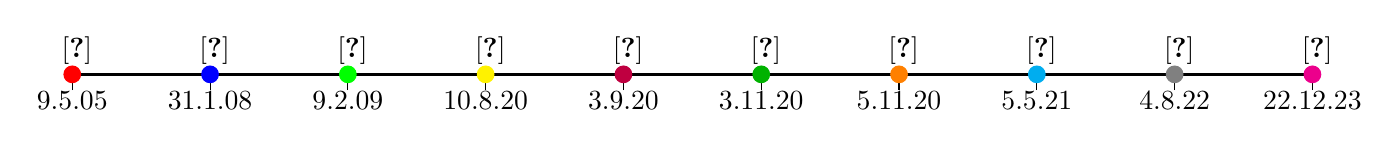
\begin{tikzpicture}
    \draw[line width=1pt] (0,0) -- (15.75,0);
    \foreach \x/\year in {0/9.5.05, 1.75/31.1.08, 3.5/9.2.09, 5.25/10.8.20, 7/3.9.20, 8.75/3.11.20, 10.5/5.11.20, 12.25/5.5.21, 14/4.8.22, 15.75/22.12.23} {
            \draw (\x,-0.2) -- (\x,0.1);
            \node[below] at (\x,-0.1) {\year};
        }
    % Articles
    \draw[red, fill=red] (0,0) circle (3pt) node[above, black] {~\cite{costello2005random}};
    \draw[blue, fill=blue] (1.75,0) circle (3pt) node[above, black] {~\cite{rudelson2008littlewood}};
    \draw[green, fill=green] (3.5,0) circle (3pt) node[above, black] {~\cite{costello2009bilinear}};
    \draw[yellow, fill=yellow] (5.25,0) circle (3pt) node[above, black] {~\cite{kwan2019algebraic}};
    \draw[purple, fill=purple] (7,0) circle (3pt) node[above, black] {~\cite{jain2020smoothed}};
    \draw[black!30!green, fill=black!30!green] (8.75,0) circle (3pt) node[above, black] {~\cite{jain2020smallest}};
    \draw[orange, fill=orange] (10.5,0) circle (3pt) node[above, black] {~\cite{campos2020singularity}};
    \draw[cyan, fill=cyan] (12.25,0) circle (3pt) node[above, black] {~\cite{jain2021singularity}};
    \draw[black!50, fill=black!50] (14,0) circle (3pt) node[above, black] {~\cite{kwan2022anticoncentration}};
    \draw[magenta, fill=magenta] (15.75,0) circle (3pt) node[above, black] {~\cite{kwan2023resolution}};
\end{tikzpicture}


\section{Random Matrices and Singularity}
The study of the singularity of random matrices is crucial because it directly impacts our understanding of system behaviors, algorithmic stability, and numerical methods across various disciplines. 
Singular matrices, which lack inverses, highlight dependencies and potential points of failure in systems and calculations (these dependencies could indicate redundancy in data, or reveal vulnerabilities in cryptographic systems). 
Investigating these singularities in random matrices helps ensure the reliability and efficiency of computational approaches, contributing significantly to advancements in theoretical and applied mathematics.




~\cite{costello2006random} The article "Random Symmetric Matrices Are Almost Surely Non-Singular"
by K. Costello, T. Tao, and V. Vu presents a significant result in the
field of random matrices. The main finding of the article is the proof
that a random symmetric matrix $ Q_n $ with independent and identically distributed 
(with the same distribution) Bernoulli variables as its upper diagonal entries
is almost surely non-singular, with a probability of $ 1-O(n^{-1/8+\delta}) $  for any $ \delta > 0 $.
This result extends previous results for random matrices to more general models of random matrices.
The article presents the history of the non-singularity problem in random matrices,
namely whether it is true that a random matrix $ A_n $ with independent Bernoulli variables
is almost surely non-singular. This question was positively answered by Komlós in 1967,
and later he generalized the result to more general models of random matrices. In a recent paper,
Tao and Vu found a different proof for random matrices that 
provides a precise estimate for the absolute value of the determinant of the matrix $ A_n $.
Building upon these previous proofs, the authors develop a quadratic version of 
Littlewood-Offord type results concerning the concentration of random variables to prove 
the non-singularity of $ Q_n $- a  random symmetric matrix.
This method allows researchers to overcome the challenge of the row and column 
transpose, which was a hurdle in previous proofs for random matrices due to the 
dependence between the row vectors of the matrix $ Q_n $.
The article raises open questions for future research in the field of random matrices:

Determinant Estimation: The article raises the question of estimating the 
determinant of random matrices. The estimation provided in the article is: $ |det\ {Q_n|=}n^{\left(1/2-o\left(1\right)\right)n} $.

Singularity Probability: Another open question raised in the article relates to estimating the 
probability that a random matrix is singular. The authors estimate that
the probability of $ Q_n $ being a singular matrix is $ {(1/2+o\left(1\right))}^n $.

The quadratic variant of the Littlewood-Offord :
Let Q be a quadratic random variable defined as: $ Q=\sum_{1\le i,j\le n}{c_{ij}z_iz_j} $  where $ z_i $
are random variables, $ {1,\ldots,n}=\ U_1\cup U_2  $
is a non-trivial partition, and S is a non-empty subset of
$ U_1 $. For each $ i\in S $, let  $d_i$  be the number of indices  $j\in U_2$ 
such that $|c_{ij}|\geq1$. If 
$ d_i\geq1$ for each $i\in S$, and I is an interval of length 1, then:
$ P\left(Q\in I\right)=O{({|S|}^{-1/2}+{|S|}^{-1}\sum_{i\in S}{d_i}^{-1/2})}^{1/4} $



\subsection{roy article1 summary}

~\cite{rudelson2008littlewood}

\subsection{Singularity Of Random Matrices}
The singularity of random matrices is a subject that sits at the intersection of probability theory, linear algebra, and theoretical computer science. It concerns the likelihood that a matrix, filled with random elements, is singular—that is, it does not have an inverse. This area of inquiry is crucial for understanding the stability of algorithms, the behavior of networks, and the foundations of statistical theory, among other applications. Researchers like Marcelo Campos, Matthew Jenssen, Marcus Michelen, and Julian Sahasrabudhe focus on advancing our knowledge about the singularity probabilities of symmetric matrices. Their efforts to refine the bounds for these probabilities and to streamline the methodologies for assessing them are essential for both theoretical insights and practical advancements in computational mathematics, physics, and engineering.\\\\

\subsubsection{Singularity Of Random Symmetric Matrices Revisited}



~\cite{campos2020singularity}
The authors improve upon previous results regarding the singularity probability of $M_n$, an $n \times n$ symmetric matrix with entries uniformly chosen from $\{\pm1\}$. They show that the probability $M_n$ is singular is at most $\exp(-c(n \log n)^{1/2})$. This result is an advancement over the previously best-known bound of $\exp(-cn^{1/2})$ Campos, Mattos, Morris and Morrison.\\\newline
The article discusses the singularity of random matrices, specifically, it addresses the singularity probability of matrices with entries from $\{-1, 1\}$, highlighting a conjecture that the probability a random $n \times n$ matrix $A_n$ is singular equals $(1 + o(1))n2^{-n+1}$, based on the likelihood of two rows or columns being identical up to sign.\\\newline
While this conjecture has seen progress over the years, with bounds on the singularity probability being improved through various mathematical advances, the paper's focus shifts to symmetric matrices. For symmetric matrices $M_n$, it's believed the singularity probability behaves similarly to the non-symmetric case, but less progress has been made. Earlier results have only shown that this probability tends to zero, without providing tight bounds.\\\newline
This paper not only offers tighter bounds on the singularity probability of $M_n$ but also argues that their method simplifies the approach taken by previous research. Specifically, they highlight an improved and simpler version of the "rough" inverse Littlewood-Offord theorem, which is crucial to their analysis. The introduction then elaborates on the techniques such as the inverse Littlewood-Offord Theorems, Fourier Analysis, Cauchy-Davenport Inequality, etc. involved in proving their main result, illustrating the complexity of dealing with "structured" versus "unstructured" vectors in the analysis of $M_n$'s singularity.\\\newline


\subsubsection{Singularity Of Discrete Random Matrices}

~\cite{jain2021singularity}
The article discusses the singularity of discrete n $\times$ n random matrices ${M_n}(\xi)$, focusing on matrices with non-constant real-valued random variables $\xi$. 
It explores the probability of singularity $ \mathbb{P}[M_n$ is singular$]=\mathbb{P}[$zero row or column$]+ (1+o_n(1))\mathbb{P}[$two equal (up to sign) rows or columns$]$ in these random matrices and confirm a conjecture related to this topic. 
They provide precise results for various scenarios, including cases involving Bernoulli distributions:\\
\textbf{For Bernoulli Distribution with} $\rho \in (0, 1/2)$:
$\mathbb{P}[M_n$ is singular$]=2n(1-\rho)^n + (1+o_n(1))n(n-1)(\rho^2+(1-\rho)^2)^2$.\\
\textbf{For Bernoulli Distribution with} $\rho \in (1/2, 1)$:
$\mathbb{P}[M_n$ is singular$]=(1+o_n(1))n(n-1)(\rho^2+(1-\rho)^2)^2$.
One key aspect of the study is the analysis of the contribution of the 'compressible' part of the unit sphere into 'structured' and 'unstructured' components to the lower tail of the smallest singular value of the matrices.
By examining this contribution, the researchers aim to gain a deeper understanding of the processes occurring in these random matrices and identify the impact of specific subsets on the singular behavior of the matrices.
In this article the novelties are:
Unlike "structured" vectors with similar components, "unstructured" vectors in random matrices have diverse values. The authors exploit this non-uniformity to analyze them. They introduce a novel "multi-slice" theorem to handle these vectors, overcoming challenges of dependence and non-integer values. This method offers a powerful tool for understanding how unstructured vectors influence the invertibility of random matrices, building upon previous work on simpler cases.


TODO::::NOT FINISHED
\\\newline\textbf{Collectively,} these articles significantly enhance the understanding of random matrix singularity, demonstrating a remarkable progression from focusing on the specific case of symmetric matrices to a broader application involving various types of discrete random matrices.
The leap from ~\cite{campos2020singularity} improved bounds and methodologies to ~\cite{jain2021singularity} resolution of longstanding conjectures and precision in probability estimates exemplifies a vibrant trajectory of research that broadens the horizon of mathematical inquiry into random matrices. 
Their findings not only underscore the complexity and richness of random matrices as a subject but also pave the way for future explorations in this captivating area of mathematics.

\subsection{Smallest Singular value of Random Matrices}

In the context of the singularity of random matrices, the smallest singular value, denoted as $s_n(A)$ for a matrix $A$, plays a crucial role. Singular values of a square $n \times n$ matrix $A$ are the square roots of the eigenvalues of $A^TA$, where $A^T$ is the transpose of $A$. These singular values are always non-negative and are often arranged in non-increasing order, so $s_1(A) \geq s_2(A) \geq \cdots \geq s_n(A)$. Here, $s_n(A)$ represents the smallest singular value.\\\\
The significance of the smallest singular value lies in its ability to provide insight into the matrix's stability and sensitivity to perturbations. Specifically, a matrix with a very small singular value is close to being singular (non-invertible), indicating that small changes in the matrix or in a linear system involving the matrix can lead to large changes in solutions or outputs. This concept is intimately related to the condition number of the matrix, defined as $\kappa(A) = \frac{s_1(A)}{s_n(A)}$, which measures how much the output value of a function can change for a small change in the input argument. A high condition number signifies potential loss of precision and numerical instability in calculations involving the matrix.\\\\
In the study of random matrices, the distribution and behavior of the smallest singular value among various classes of random matrices are of significant interest. This analysis aids in understanding the invertibility of these matrices and their robustness to perturbations, impacting numerical methods, signal processing, and data science, among other fields. Establishing bounds on the probability that the smallest singular value of a random matrix falls below a certain threshold is particularly relevant. Such bounds offer insights into the likelihood of a random matrix being nearly singular or well-conditioned, thereby affecting the reliability of computations performed with these matrices.\\\


\subsubsection{Smoothed Analysis Of The Smallest Singular Value With Discrete Noise}


~\cite{jain2020smoothed}

In the context of numerical linear algebra and random matrix theory,
the behavior of the smallest singular value of matrices under random
perturbations has been a subject of extensive study due to its profound
implications on matrix invertibility and stability of numerical algorithms.
Recent advancements by Vishesh Jain, Ashwin Sah, and Mehtaab Sawhney have 
shed new light on this topic, that extend and challenge previous
understandings.

The researchers have provided a comprehensive analysis that generalizes
the bounds on the probability of a matrix being near-singular after
random perturbation. Specifically, they have shown that for a matrix
${A}$ perturbed by a random matrix 
${M}$ with i.i.d. sub-Gaussian entries, the smallest singular value
of ${A+M}$ remains unlikely to be negligible. This result is significant
as it relaxes the stringent requirements previously believed necessary,
suggesting a broader class of matrices maintains stability under
perturbations.

A novel theoretical contribution of this work is the establishment 
of sharp lower bounds on the smallest singular value for matrices
subjected to discrete noise perturbations. This finding contradicts
the speculation by renowned mathematicians Terence Tao and Van Vu,
demonstrating that the influence of certain parameters on the smallest
singular value is inherently limited. This insight not only deepens our
theoretical understanding but also has practical ramifications in 
the design and analysis of algorithms.

The study's approach combines geometric
analysis with probabilistic methods, a technique
that has allowed the authors to navigate the complex landscape
of high-dimensional matrices and their perturbations.
By innovatively applying these methods, 
the authors have been able to uncover patterns and bounds
that were previously obscured.

 

\subsubsection{On The Smallest Singular Value Of Symmetric Random Matrices}

~\cite{jain2020smallest}
In this article the authors explores the behavior of the smallest singular value in n $\times$ n random symmetric matrices  $A_n(ij) = A_n(ji)$. 
They investigate $M_n$ random matrix $n\times n$ each of the entries is an independent copy of a sub-Gaussian random variables $\xi$ with mean $0$ and variance $1$.
The smallest singular value of $M_n$ is denoted as $s_n(M_n)$, defined as: $s_n(M_n) = inf_{v \in \mathbb{S}^{n-1}} \|Mv\|_2$ where $\mathbb{S}^{n-1}$ is the unit sphere in $\mathbb{R}^n$ \textbf{(from The Littlewood-Offord problem and invertibility of random matrices)}.
The main result shows that for a random symmetric matrix $A_n$ with sub-Gaussian entries, the probability of $s_n(A_n)$ being less than $\epsilon/\sqrt{n}$ is bounded by: $P[s_n(A_n)\leq \epsilon/\sqrt{n}]\leq C \epsilon^{1/8}+2e^{-c n^{1/2}}$ for all $\epsilon \geq 0$, where $C$ and $c$ are constants depending on the sub-Gaussian norm of $\xi$.
When $\xi$ is a Rademacher random variable, the probability bound becomes: $P[s_n(A_n) \leq \epsilon / \sqrt{n}] \leq O(\epsilon^{1/8}+ \exp(-\Omega((\log{n})^{1/4}n^{1/2})))$
It also mentions the Median Regularized Least Common Denominator (MRLCD) and the Median Threshold.
These notions improve upon the Regularized Least Common Denominator (RLCD) by efficiently utilizing the arithmetic structure of vectors, particularly when many projections of a vector are arithmetically unstructured.
They demonstrate that the MRLCD and median threshold have level sets that can be covered by sufficiently small nets at the appropriate scale, which is crucial for their applications. 
These new concepts can replace RLCD in various applications and are expected to provide better quantitative estimates. 
 
\\\newline\textbf{The authors} of the article On the smallest singular value of symmetric random matrices ~\cite{jain2020smallest} extended the work on the smoothed analysis of the smallest singular value ~\cite{jain2020smoothed}, particularly in contexts involving discrete noise. 
Their research builds upon and broadens previous findings by offering new insights into how the smallest singular value of a matrix behaves when perturbed by noise, including discrete types. 
Their contributions include relaxing the conditions required for analyzing the stability of matrices under perturbations and introducing novel methods to study the effects of noise, thereby enhancing the theoretical framework that underpins the smoothed analysis in numerical linear algebra.\\
Their work notably advances the understanding of matrix perturbations beyond the contributions of earlier researchers such as Rudelson and Vershynin, who had established foundational results in the area of random matrices and their singular values. By focusing on less restrictive conditions and exploring the role of discrete noise, Jain, Sah, and Sawhney not only refine the bounds on the smallest singular value but also elucidate the practical implications of their findings for the performance and robustness of numerical algorithms. This relationship between their work and that of their predecessors underscores a significant progression in the field, driving forward the applicability of smoothed analysis to a wider range of problems and algorithms.
\subsection{Overview}
The body of work presented in the featured articles systematically explores the behavior of random matrices, particularly focusing on the singular probability and the smallest singular value of symmetric matrices, Bernoulli matrices, and matrices with discrete noise. Initially, foundational conjectures and optimal tail probability estimates for the smallest singular value set the stage for a deep dive into the peculiarities of random matrices with independent entries. 
Progressing chronologically, the research delves into the singular probabilities of symmetric matrices, significantly improving upon previous bounds and introducing simpler methodologies. 
This exploration is further enriched by addressing the singularity of discrete random matrices, not only confirming a long-standing conjecture for Bernoulli matrices but also extending the results to matrices with uniform support distributions. 
The series of articles culminates in offering generalizations that extend these insights to a wider class of polynomials and variables, showcasing the robustness of the methodologies developed. Through a combination of refining existing techniques and expanding the scope of inquiry, this collective research elucidates the intricate behaviors of random matrices, marking a significant advancement in our understanding of their properties and establishing a chronological progression of knowledge.

\newpage
\section{Littlewood-Offord}

The Littlewood-Offord problem matters because it provides foundational insights into the probability distributions of linear combinations of random variables, and is crucial for understanding the stability and invertibility of random matrices as we saw in the previous section. The following articles expand our understanding of its implications for higher degree polynomials, particularly in bilinear and quadratic forms.

\subsection{Bilinear and Quadratic variants on the Littlewood-Offord problem}

Costello's paper~\cite{costello2009bilinear} presents extensions of the Littlewood-Offord problem and related results to polynomials of higher degree, in particular bilinear and quadratic forms.

They presented the history regarding the problem in its linear form specifically noting Halász's extension, which bounds the probability that the sum of vectors in \(R^d\), each multiplied by independent complex-valued random variables, equals a specific value, under the condition that no proper subspace contains too many of these vectors.

They highlighted the work of Kahn, Komlos, and Szemeredi, which utilized the concept to demonstrate that the singularity probability of a matrix is exponentially small relative to its size. Furthermore, Tao and Vu, along with Rudelson and Vershynin, confirmed this observation by showing that if the sum assumes a single value with a probability of at least \(n^{-c}\) for some fixed \(c\), then the coefficients must originate from a short generalized arithmetic progression.
\newline
\vspace{-0.6\baselineskip}

Their first main result shows is that every bilinear form with sufficiently large concentration probability is in some sense close to this degenerate example.\\
\vspace{-0.6\baselineskip}

The theorem establishes that for bilinear forms \(x^T A y\) with high concentration probabilities, where \(x\) and \(y\) are random vectors with entries chosen from \(\{1, -1\}\), the coefficient matrix \(A\) must contain a large rank-one submatrix if each row has a sufficient number of nonzero entries. This condition holds true even when the function \(f(y)\), determining the concentration level, is constant or when \(y\)'s entries have probabilities altered to include zeros.\\
\vspace{-0.6\baselineskip}

The next theorem addresses the concentration of quadratic forms \(x^T A x\), where \(x\) is a vector of random variables and \(A\) is a symmetric matrix with a significant number of nonzero entries in each row. It establishes that the probability of the quadratic form equaling a linear form \(L(x)\) plus a constant \(c\) is bound by a function of \(r\), the minimum number of nonzero entries per row, suggesting a dispersion characteristic that becomes more pronounced as \(r\) increases. This theorem applies even when the linear form \(L(x)\) is zero, illustrating the broad applicability of the result to understanding the dispersion of quadratic forms involving random variables.\\
\vspace{-0.6\baselineskip}

Costello's extensions provide as the basis to further expansion of the understanding of quadratic variants of the Littlewood-Offord problem.


~\cite{kwan2023resolution}


\section{Random Graphs}



~\cite{kwan2023anticoncentration}






\textbf{Background:}\\
- Quadratic Polynomial Concentration: Consider a quadratic polynomial
in ${n}$ independent Rademacher random variables 
${\xi_1, \xi_2,...,\xi_n}$ meaning ${Pr(\xi_i=1)=Pr(\xi_i=-1)=0.5}$ 
for each ${i}$:
$${f(\xi)=\sum_{i,j=1}^{n} a_{ij} \xi_i \xi_j + \sum_{i=1}^{n} b_i \xi_i + c}$$
where ${a_{ij},b_i}$ and ${c}$ are coefficients,
and the polynomial is said to exhibit significant 
concentration if for some value ${x}$, the probability
${Pr(\xi=x)}$ exceeds a certain threshold, indicating 
that ${f(\xi)}$ is closely concentrated around ${x}$.

- Point Probability: Can be represented as ${P(f(\xi_1, \xi_2,...,\xi_n) = k)}$ where ${k}$ is a specific value.
- Ramsey's theorem states that for any given integers ${r}$ and ${s}$,
there exists a least integer ${N=R(r,s)}$ 
such that any graph on ${N}$ or more vertices,
no matter how its edges are colored using two colors
(say, red and blue), will contain either a red clique of size ${r}$
or a blue clique of size ${s}$.
A clique here refers to a subset of vertices such that every two distinct
vertices are connected by an edge.

The article introduces inverse theorems of a similar flavour to Costello's
conjecture, showing that if a quadratic polynomial exhibits point
probabilities significantly larger than ${1/n}$,
it must be close to a low-rank quadratic form.
This is achieved through a detailed analysis
involving the arrangement of coefficients
and the algebraic structure of the polynomial.

The authors in the given paper focused on the quadratic
Littlewood-Offord problem by examining the concentration
of quadratic polynomials in independent Bernoulli random
variables. They extended classical questions about linear
polynomials to the quadratic case, exploring the
conditions under which a quadratic polynomial can have
significant point probabilities. Their main results,
as summarized in Theorems 1.1 and 1.2, establish a connection
between the anti-concentration of a quadratic polynomial 
$f(\xi)$ and the algebraic structure of $f$.
In particular,
they demonstrated that if a quadratic polynomial has a 
concentration probability significantly
larger than $\frac{1}{n}$, it must be close to
a quadratic form with low rank.

\subsubsection{Quadratic Approximation Bound}
In \textbf{Theorem 1.1}, for any given $r \geq 3$ and
$0 < \epsilon \leq 1$, they identified a constant
$C = C(r, \epsilon)$ such that for a quadratic polynomial
$f \in F[x_1, \dots, x_n]$ (where $F$ is either 
$\mathbb{C}$, $\mathbb{R}$, or $\mathbb{Q}$) with all coefficients
of absolute value at most 1, and
$\xi = (\xi_1, \dots, \xi_n) \in \text{Rad}^n$, if
${\sup_{x \in F} \Pr(f(\xi) = x) \geq C \cdot \frac{(\log n)^{r/2}}{n^{1-2/(r+2)}}}$,
then there exists a quadratic form
$h \in F[x_1, \dots, x_n]$ of rank strictly less than $r$
such that the sum of the absolute values of the coefficients
of $f - h$ is at most $\epsilon n^2$.
 
Theorem 1.1 provides a significant breakthrough in this 
area by demonstrating that if a quadratic polynomial shows 
point probabilities significantly larger than $1/n$, then
it closely resembles a quadratic form of low rank.
This finding is profound because it not only generalizes
the Littlewood-Offord problem to quadratic polynomials
but also introduces an "inverse" aspect to the problem

\subsubsection{Constrained Coefficient Approximation}
\textbf{Theorem 1.2} follows a similar line of reasoning but
focuses on the scenario where the quadratic polynomial ${f}$'s 
degree-2 coefficients come from a specific set $S$. 
It states that under similar conditions of anti-concentration,
there exists a quadratic form $h$ close to ${f}$,
differing in at most $\epsilon n^2$ coefficients, 
and also has a rank strictly less than $r$. 
This theorem further advances the generalization of the 
Littlewood–Offord problem to quadratic polynomials,
not just by considering the concentration probabilities
of these polynomials on single values, but also by imposing
an additional structural constraint on the coefficients.

These theorems can provide stronger anti-concentration
estimates for certain complex quadratic polynomials,
particularly those not easily factorizable over $\mathbb{C}$,
as previously conjectured by Costello.
It is noted that for complex quadratic forms with a rank
of at most 2, which can be expressed as a sum of squares 
of linear forms, these invariably factorize into linear factors
in $\mathbb{C}$.
Thus, applying Theorems 1.1 and 1.2 with $r = 3$ suggests
that if a polynomial $f(\xi)$'s point probabilities
significantly exceed $n^{-3/5}$, it implies the existence 
of a closely related quadratic form $h$, which factorizes
into linear factors over the complex numbers.

Beyond the theoretical advancements, this paper extends
its findings to the study of Ramsey graphs,
specifically addressing and providing asymptotic 
answers to questions previously posed by Kwan, Sudakov, and Tran.

\subsubsection{Edge Anti-Concentration in C-Ramsey Graphs}
In C-Ramsey graphs as previously described at~\ref{sec:anticoncentration}
must in some sense resemble random graphs,
and this belief has been supported by a number of theorems
showing that certain `richness' properties
characteristic of random graphs hold for all C-Ramsey graphs.
The first result of this type was due
to Erdos and Szemerédi~\cite{erdHos1972ramsey}

The aforementioned Erdos–Szemerédi theorem can be
interpreted as a (weak) “concentration” theorem:
the numbers of edges in induced subgraphs cannot
be “too extreme"

However, on the contrary, there exists 
a body of research that demonstrates 
the extreme perspective.Kwan, Sudakov and Tran
~\cite{kwan2019anticoncentration}
asked about anti-concentration of the
edge distribution in Ramsey graphs.
Specifically, for an n-vertex C-Ramsey graph,
let X be the number of edges induced by a uniformly 
random set of $n/2$ vertices. Is it true that
$Pr(X=x)=O(1/n)$ for all $x \in N$?
understanding could improve proofs for 
conjectures about the edge distribution in such graphs.
Using Theorem 1.2, they also addressed 
Kwan, Sudakov, and Tran's question by representing X
as a quadratic polynomial and proving that 
Ramsey graphs are too disordered for this 
polynomial to approximate a low-rank quadratic form.


\textbf{Theorem 1.3.} The following holds for any fixed constants
$C, c > 0$. Let $G$ be an $n$-vertex $C$-Ramsey graph, and, 
for some $cn \leq k \leq (1 - c)n$, let $X$ be the number of edges
induced by a uniformly random subset of $k$ vertices of $G$.
Then for any $x \in \mathbb{Z}$, $we have \Pr(X = x) \leq n^{o(1)-1}$.
This theorem directly applies the insights gained from 
Theorems 1.1 and 1.2 to the context of Ramsey graphs, 
offering a novel perspective on edge statistics within these graphs.
A C-Ramsey graph is defined as a graph that avoids large homogeneous
subsets (i.e., large subsets of vertices that are either all
connected or all disconnected), which is a central theme
in Ramsey theory. The theorem investigates the anti-concentration of edge counts in such graphs by considering the number of edges ($X$) within a randomly selected subset of vertices.
Specifically, for an $n$-vertex C-Ramsey graph and a subset
of vertices of size between $cn$ and $(1-c)n$,
Theorem 1.3 establishes that the probability of exactly $x$ edges
being induced within this subset is bounded above by $n^{o(1)-1}$
for any integer $x$. This result implies a high level of 
anti-concentration of edge counts, indicating that in a C-Ramsey graph,
the distribution of the number of edges in subsets of vertices
does not significantly concentrate around any specific number.
Such a behavior mirrors one of the properties expected in random
graphs, where edge counts among subsets of vertices are distributed
broadly without significant concentration.

By linking the algebraic properties of quadratic polynomials
to the structure of Ramsey graphs, Theorem 1.3 showcases how 
abstract algebraic concepts can have concrete applications in graph theory.

This application highlights the interplay between discrete
mathematics and algebraic probability, demonstrating the 
practical relevance of algebraic characterizations of 
quadratic polynomials in understanding the structure 
and randomness inherent in Ramsey graphs. 
By analyzing the edge counts within Ramsey graphs 
through the framework of quadratic polynomials—using 
entries from the graphs' adjacency matrices—the study 
delves into the anti-concentration properties of these graphs.
For a Ramsey graph $G$ with an adjacency matrix $A$, 
the investigation into the edge counts of randomly chosen
vertex subsets reveals insights into the graph's structure,
making to the properties observed in random graphs.
The researchers applied principles from the quadratic 
Littlewood–Offord problem to explore the distribution 
of edge counts in subsets of vertices within C-Ramsey graphs.
They focused on determining whether, 
for a randomly selected subset of $n/2$ vertices in an
$n$-vertex C-Ramsey graph, the probability that the induced
subgraph contains exactly $x$ edges adheres to $O(1/n)$ 
for all $x$. Such a finding would suggest that the edge 
distribution in Ramsey graphs does not overly concentrate 
around any specific edge count, reflecting a characteristic
commonly associated with random graphs.

\subsection*{Overview}





\section{Overview}
The studies presented in this document have led to significant progress
in understanding the behavior of random matrices and in improving the 
tools and techniques for their analysis.
They refer to the Littlewood-Offord theory as a basis
for comprehending the singularity properties of random matrices,
offer tools and models for analyzing the singularity of matrices,
and allow researchers to more accurately evaluate the behavior of
matrices in random environments. Consequently,
the articles substantially enhance the understanding of the behavior of random matrices.
The advanced knowledge in the field enables
researchers and scientists to deepen their
understanding of the mathematical and singular
properties of random matrices, 
facilitating their application across a diverse array of fields.


\newpage
\printbibliography

\end{document}
